\documentclass[conference]{IEEEtran}

\usepackage{xspace}
\usepackage{enumitem}
\usepackage{multirow}
\usepackage{graphicx}
\usepackage{comment}
\graphicspath{{figs/}}
\DeclareGraphicsExtensions{.pdf,.jpeg,.png}

% todo notes
\usepackage[colorinlistoftodos]{todonotes}
\newcommand{\TODO}[1]{\todo[inline, color=yellow!40]{#1}}

\begin{document}
\title{A Year in the Life of a Parallel File System}

\begin{comment}

\author{\IEEEauthorblockN{Glenn K. Lockwood, Teng Wang, Suren Byna, Nicholas J. Wright}
\IEEEauthorblockA{Lawrence Berkeley National Laboratory\\\{glock,tengwang,sbyna,njwright\}@lbl.gov
}
\and
\IEEEauthorblockN{Shane Snyder, Philip Carns}
\IEEEauthorblockA{Argonne National Laboratory\\
\{ssnyder,carns\}@mcs.anl.gov}
}
\end{comment}

% aliases so we can swap terms out for double-blind
\newcommand{\tokio}{TOKIO\xspace}
\newcommand{\tokiolong}{Total Knowledge of I/O\xspace}
\newcommand{\nersc}{NERSC\xspace}
\newcommand{\nersclong}{National Energy Research Scientific Computing Center\xspace}
\newcommand{\alcf}{ALCF\xspace}
\newcommand{\alcflong}{Argonne Leadership Computing Facility\xspace}
\newcommand{\cori}{Cori\xspace}
\newcommand{\edison}{Edison\xspace}
\newcommand{\mira}{Mira\xspace}
\newcommand{\mirafsone}{mira-fs1\xspace}
\newcommand{\scratchone}{scratch1\xspace}
\newcommand{\scratchtwo}{scratch2\xspace}
\newcommand{\scratchthree}{scratch3\xspace}
\newcommand{\cscratch}{cscratch\xspace}

\maketitle

% As a general rule, do not put math, special symbols or citations
% in the abstract
\begin{abstract}

Lorem ipsum

\end{abstract}

\section{Introduction}

I/O performance variation has been studied extensively, and a variety of conditions have been identified as contributing factors to poor I/O performance.  Most studies have focused on enumerating the sources of I/O performance loss at a single point in time, assuming that performance loss is a transient effect due to contention from other jobs.  However, recent work~\cite{Lockwood2017} has shown that performance variation can occur over periods of days as a result of systematic, longer-term conditions of a storage system.
%
Overall performance (and thus scientific productivity) can be improved for a
wide range of users if these deviations can be identified and attributed
quickly in production.

%Such systematic, long-term I/O performance variation remains much less well understood despite its relevance to scientific campaigns that may experience uneven throughput or resource consumption over the course of months or years.  In this work, we differentiate \emph{long-term performance variation} from \emph{short-term performance variation} and characterize the factors that contribute to long-term performance variation on a diverse range of large-scale production parallel storage systems.

A number of recent efforts~\cite{Lockwood2017,Vazhkudai2017guide,Agelastos2014ldms,Kunkel2014siox} have advanced the
state of the art in scalable data collection, making it possible to observe
production systems at unprecedented scales.  It remains an open problem,
however, how go best interpret this data to quickly for maximum production
impact, and what types of instrumentation have the greatest return on
investment.

We investigate this issue by studying performance data collected from
large parallel file systems at NERSC and the ALCF over the course of
a year of production use.  We capture not only system monitoring data, but also
application-level instrumentation as well as daily performance results from a set of representative I/O benchmarks which we use as active file system performance probes. The breadth of
this data set enables us to investigate performance variation over
multiple time scales, ranging from days to weeks, and allows us insight
into how often performance loss is observed over longer periods of time.
The depth of this data set enables us to observe how system behavior is
reflected in user-perceived performance and how combinations of factors
contribute to overall performance.

We also develop a methodology for identifying inflection points in
long-term user-perceived performance due to factors beyond their control,
such as hardware failures, software changes, capacity constraints, or
contention.  These trends are easily overlooked or misattributed given the
complexity and inherent variability of the I/O system itself, but can have a
significant long term impact on efficiency.  Once an inflection point has
been found, we investigate methods for guiding administrators to likely
contributing factors if not outright identifying definitive root causes for
anomalous performance.

%By integrating holistic I/O monitoring throughout the
%year-long experiment, we then quantitatively show
%that common sources
%of short-term variation, such as bandwidth or metadata contention,
%play less significant role in long-term performance variation.
%Given this multiscale nature of I/O performance variation, we conclude that the probabilistic effects of transient interference \emph{and} the autocorrelative effects of long-term variation are required to capture the full picture of performance variation on parallel storage systems.

The primary contributions of this paper are as follows:
\begin{itemize}
\item \TODO{fill in firm contributions as we nail down outcomes, see text in latex comments}
\item \TODO{could be findings about the nature of file system performance
(especially things that notably diverge from expectations),
methodologies for analyzing data, recommendations for instrumentation
techniques, or recommendations for system administration}
\end{itemize}

%The remainder of the paper is organized as follows.  \TODO{Fill in}


\section{Related Work} \label{sec:related}

Several recent studies have contributed techniques to combine
systemwide HPC instrumentation data for integrated
analysis~\cite{Lockwood2017,Vazhkudai2017guide,Agelastos2014ldms,Kunkel2014siox,RIOT_2013}.
Vazhkudai et al. notably used a Splunk data warehouse to analyze system
logs and perform operational analytics on a large-scale storage system~\cite{Vazhkudai2017guide}.
The cloud computing community has also identified the need to unify
analysis capabilities across diverse environments.
The Dapper system
developed by Sigelman et al. combines comprehensive tracing with a novel
sampling method to observe critical paths in large cloud environments in great
detail~\cite{Sigelman2010dapper}.

Luu et al.~\cite{Luu:2015:HPDC} studied application I/O logs from multiple platforms to derive conclusions on I/O system utilization and library usage.
Di et al.~\cite{7973730} and Park et al.~\cite{Park2017BigDM} have
investigated performing correlation analysis on HPC log data once it has been
collected.  Their analyses included compute and network resources, with a
particular emphasis on event logs. Inacio et al. analyzed performance variability using statistical analysis of file system read/write operations and concluded that both the experimental environment and Lustre stripe settings impact performance applications. 
Others have documented 
I/O performance variability anecdotes on leadership-scale
systems~\cite{Lofstead2010,Yildiz2016,carns2011understanding} and proposed
methods to combat it.  

However, these studies of application I/O and parallel file system performance and variability are based either on a small set of applications or on observations over a short duration.
Furthermore, examining how performance and variation may change over time remains relatively unexplored, with the existing body of work being largely anecdotal~\cite{Haryadi2018fail}.
In this work, we build upon best-in-class previous efforts by combining system monitoring, application monitoring, and active performance probing
to quantify holistically how I/O performance variation manifests across many dimensions over a year-long period.
To this end, we also introduce systematic methods to help automate the task of deriving actionable insight from these data sources over multiple time scales.
We have analyzed these holistic data sets for an entire year on multiple parallel file systems and present a broad statistical analysis that provides an unprecedented advancement in our understanding of HPC I/O performance variability.

\section{Methodology}\label{sec:methods}

Previous studies have demonstrated the feasibility of 
holistic HPC I/O analysis and used it to observe anomalous I/O behavior and
contributing factors over short time scales\cite{Lockwood2017}. This methodology was later formalized in the specification of the \tokio (\tokiolong) framework~\cite{Lockwood2018tokio}. 
In this work, we use 
%the \tokio 
a similar
methodology to collect and analyze a complete
year of I/O metrics on multiple production platforms.  This section
summarizes the \tokio framework, 
describes the production HPC platforms that we have 
%deployed it on, 
used in this study,
and introduces our methodology for active probing of storage system
performance.

\subsection{Data collection framework}\label{sec:methods/tokio}

%A holistic approach to understanding I/O behavior is a necessity given the move towards more complicated I/O architectures (in terms of number of constituent components, like high-level I/O libraries, I/O middleware systems, and low-level storage hardware) on these systems. \tokio's primary goal is to arm system users, administrators, and I/O researchers with the necessary tools to navigate this complexity and to make meaningful observations into how workloads interact with the I/O subsystem.

\tokio is a framework facilitating holistic characterization and analysis of I/O workloads running on today's production HPC systems. Conceptually, it provides an abstraction layer between component-level monitoring tools already deployed on HPC platforms and higher-level I/O analysis tools that utilize this data. The fundamental roles of the \tokio framework are to: collate monitoring data from distinct components; integrate and normalize the data from these components; and present coherent interfaces for indexing and accessing this data.
\TODO{Maybe a simple component diagram is useful if we have the space -SS}

\tokio uses a modularized software architecture and a generic data format
specification for system monitoring data, simplifying portability to new HPC
platforms. Software modularity is accomplished by defining abstract
\textit{connectors} to monitoring sources, each exposing interfaces for
extracting relevant data in a format suitable for \tokio.  A generic
timeseries format is used for semantically consistent access to data
originating from distinct monitoring tools, even though each tool uses its
own underlying data format with its own scope and granularity.
The timeseries data format designates a number of metrics
that are common to classes of monitoring components.  For example, file system
monitoring tools often gather common metrics such as read/write bandwidths
and operation counts. \tokio connectors can convert the native data formats
of their underlying tools to this generic format in-memory as part of
on-demand analysis, or \tokio-aware tools can archive directly into this
format on-disk. These design decisions greatly simplify the process of
integrating new monitoring sources as well the process of developing
platform-independent I/O analysis tools.  This study in particular relies on
integrated analysis of the following monitoring modules:

\begin{itemize}[leftmargin=*]
\item \textbf{Application-level monitoring}: \textit{Darshan}~\cite{Carns2009} is an application I/O characterization tool that is commonly deployed at production HPC facilities. It provides a condensed set of I/O counters, timers, and other statistics for each file accessed by a given application.

\item \textbf{File system workload monitoring}: \textit{LMT}~\cite{lmt} and \textit{ggiostat}~\cite{Lockwood2017} are examples of 
production-quality file system monitoring tools for Lustre and GPFS deployments, respectively. These tools each periodically capture metrics quantifying file system workloads over a given time interval, with some of these metrics being common to both tools (e.g., observed read/write bandwidths, number of specific I/O operations issued, etc.) and other metrics being file system specific (e.g., the CPU utilization on a given Lustre metadata server captured by LMT).

\item \textbf{File system capacity/health monitoring}: File system specific tools like Lustre's \textit{lfs} and \textit{lctl} or GPFS's \textit{mmdf} and \textit{mmlsdisk} can be invoked periodically to capture current file system state, including the capacity and failover status of individual storage servers and/or disks in the system.

\item \textbf{Job scheduler monitoring}: Job schedulers like Slurm~\cite{2003slurm} often keep a detailed accounting of all jobs that execute on a particular system, including useful details like the size of the job and its placement across available compute nodes.
\end{itemize}

The telemetric data from these monitoring modules are aggregated into \emph{attributes} associated with each job, and all of the attributes associated with a job are represented as \emph{feature vectors}.
Wherever possible, attributes are also represented as \emph{coverage factors}~\cite{Lockwood2017} which quantify the fraction of system-wide activity that can be attributed to the job of interest.
For example, a job's \emph{bandwidth coverage factor} is the number of bytes read and written by that job's application (measured by Darshan) divided by the number of bytes read and written across the entire parallel file system (measured by LMT or ggiostat) while that job was running.
A coverage factor of 1.0 indicates that a job was the exclusive consumer of
a resource, while a coverage factor of 0.4 indicates that other competing
jobs consumed 60\% of the total delivered resources.  Each job in this study
typically produces a feature vector with 220 attributes including derived
values.  The exact size of the feature vector depends on what monitoring
modules are available on the target platform at the time the job is
executed.

\subsection{Platforms}\label{sec:methods/platforms}

% Please add the following required packages to your document preamble:
% \usepackage{multirow}
\begin{table}
\centering
\caption{Description of \nersc and \alcf test platforms.}
\label{tab:platform-descriptions}
\begin{tabular}{|c|c|c|c|c|}
\hline
                                                                                   & \textbf{Platform}                                                              & \textbf{FS Name (Type)} & \textbf{Size} & \textbf{Peak Rate}     \\ \hline
\multirow{3}{*}{\textbf{\begin{tabular}[c]{@{}c@{}}\edison\\ (\nersc)\end{tabular}}} & \multirow{3}{*}{\begin{tabular}[c]{@{}c@{}}Cray XC30\\ 5,586 CNs\end{tabular}} & \scratchone (Lustre)               & 2.2 PiB       & 48 GB/sec              \\ \cline{3-5} 
                                                                                   &                                                                                & \scratchtwo (Lustre)               & 2.2 PiB       & 48 GB/sec              \\ \cline{3-5} 
                                                                                   &                                                                                & \scratchthree (Lustre)               & 3.3 PiB       & 72 GB/sec              \\ \hline
\textbf{\begin{tabular}[c]{@{}c@{}}\cori\\ (\nersc)\end{tabular}}                    & \begin{tabular}[c]{@{}c@{}}Cray XC40\\ 12,076 CNs\end{tabular}                 & \cscratch (Lustre)               & 28 PiB      & 744 GB/sec \\ \hline
\textbf{\begin{tabular}[c]{@{}c@{}}\mira\\ (\alcf)\end{tabular}}                     & \begin{tabular}[c]{@{}c@{}}IBM BG/Q\\ 49,152 CNs\end{tabular}                  & \mirafsone (GPFS)               & 7.0 PiB       & 90 GB/sec              \\ \hline
\end{tabular}
\end{table}

We deployed \tokio on the \edison and \cori systems at \nersc and the \mira system at the \alcf. Each of these platforms, along with their corresponding file systems analyzed as part of this study, are briefly described in Table~\ref{tab:platform-descriptions}.

Darshan is installed and automatically enabled on each of these systems, transparently characterizing the I/O workloads of a large portion of  each system's job population. 
\nersc has deployed LMT for full-time monitoring of the Lustre scratch
volumes on both \edison and \cori, while the \alcf has deployed ggiostat to
do the same for the GPFS volumes on \mira.
\nersc systems additionally utilize the Slurm job scheduler, which allows for the capture of detailed metadata for every job executed on \edison or \cori.
\tokio uses these data sources in-place to provide a unified holistic view
of I/O performance without copying data to a dedicated database facility.

\subsection{I/O Performance Probes}\label{sec:methods/benchmarks}

\begin{table}
\centering
\caption{I/O Performance Probe Motifs}
\label{my-label}
\begin{tabular}{|r|c|c|}
\hline
\multicolumn{1}{|l|}{}    & \begin{tabular}[c]{@{}c@{}}$O(10^1 \textup{ MiB})$\\\textbf{Transfers}\end{tabular} & \begin{tabular}[c]{@{}c@{}}$O(10^2 \textup{ MiB})$\\\textbf{Transfers}\end{tabular} \\ \hline
\textbf{Shared File}      & IOR/shared                 & VPIC and BDCATS              \\ \hline
\textbf{File Per Process} & IOR/fpp                    & HACC                         \\ \hline
\end{tabular}
\label{tab:benchmark-motifs}
\end{table}

To measure the performance variation on the systems described in Section \ref{sec:methods/platforms}, we ran four I/O-intensive benchmarks on a daily basis from February 14, 2017 to February 15, 2018.
We utilize these benchmarking runs as another ad-hoc monitoring source for this study, actively probing the I/O performance of each analyzed file system on a daily basis across a range of representative I/O motifs.
The four underlying benchmarks (VPIC, BDCATS, HACC, and IOR) were chosen to exercise a variety of I/O workloads and covered the four I/O motifs listed in Table \ref{tab:benchmark-motifs} in both read and write modes.
Each application was configured to run identically to previous work~\cite{Lockwood2017} with the goal of using a substantial fraction of the I/O subsystem's peak bandwidth while using minimal production cycles.
All probes ran using 256 nodes (4,096 processes) on \cori, 128 nodes (2,048 processes) on \edison, and 1,024 nodes (16,384 processes) on \mira.
Data was striped as widely as possible in all cases; this corresponds to striping over every OST (for \cori and \edison) or every LUN and using the eight I/O nodes allocated to each job (for \mira).

The resulting 366-day experiment generated 11,986 performance observations across \mira, \cori, and \edison, reflecting 81.9\% of the intended probes having generated results.
The remaining 18.1\% of missing probes resulted from system downtime, malfunctions of component-level monitoring tools or the automated test scheduling, queue wait times that exceeded 24 hours, and benchmarks exceeding their walltime.
The fact that no results were obtained for jobs that ran so slowly that they exceeded their reserved walltime is significant in that this dataset does not capture the absolute worst performance observed.
Although not ideal, this reflects the realities of daily testing on production systems.

%\TODO{Add details of the number of processes the benchmarks ran with, and how the file systems are set up, i.e., number of OSTs on \cori, number of I/O nodes used on \mira 
%\\
%\edison was mentioned in the previous paragraph; Figure 1 doesn't have the results. -- Suren}
% DONE - 2018-03-26 gkl


\section{Identifying Trends}  \label{sec:features}

\begin{figure}
    \centering
    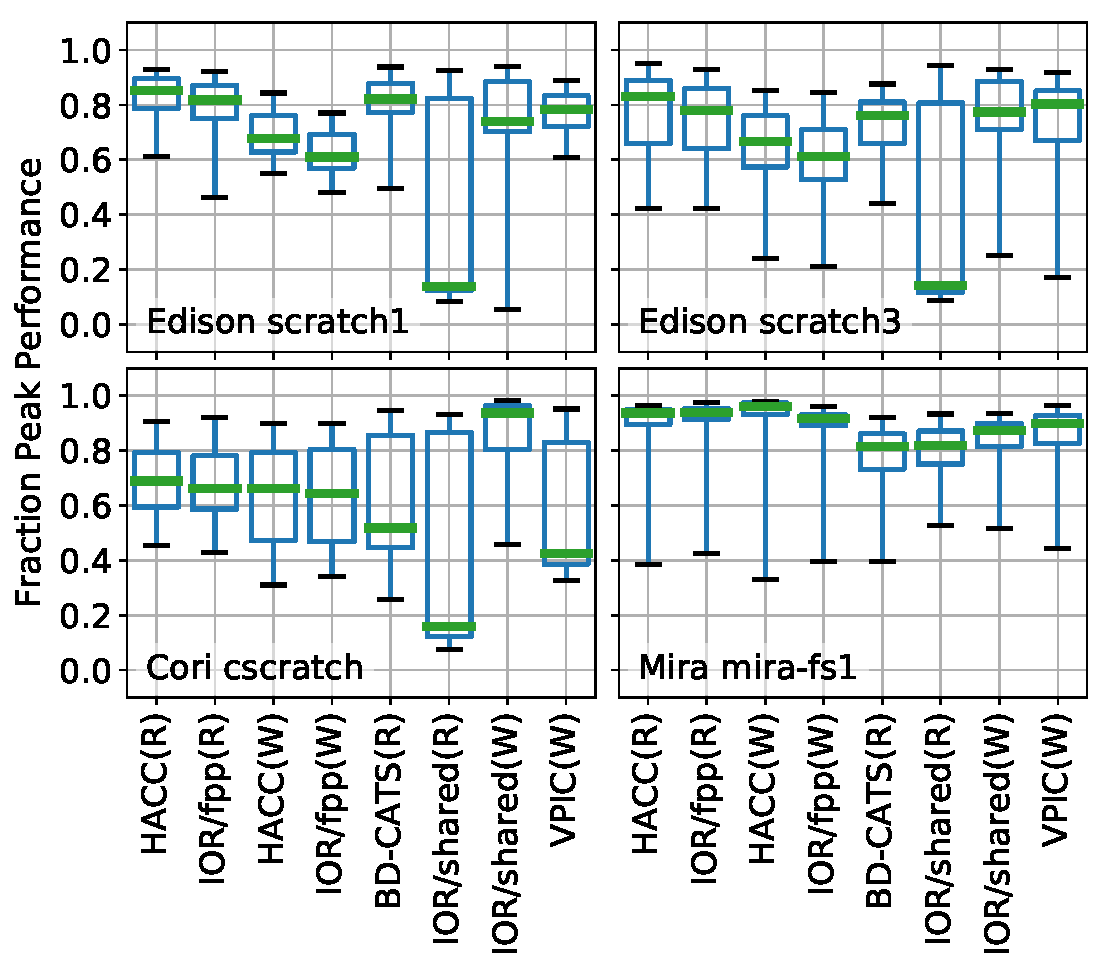
\includegraphics[width=0.9\columnwidth]{summary-boxplots}
    \vspace{-.15in}
    \caption{I/O performance grouped by test applications and read(R)/write(W) mode.  Whiskers represent the 5th and 95th percentiles.}
    \label{fig:summary-boxplots}
\end{figure}

\begin{figure*}
    \centering
    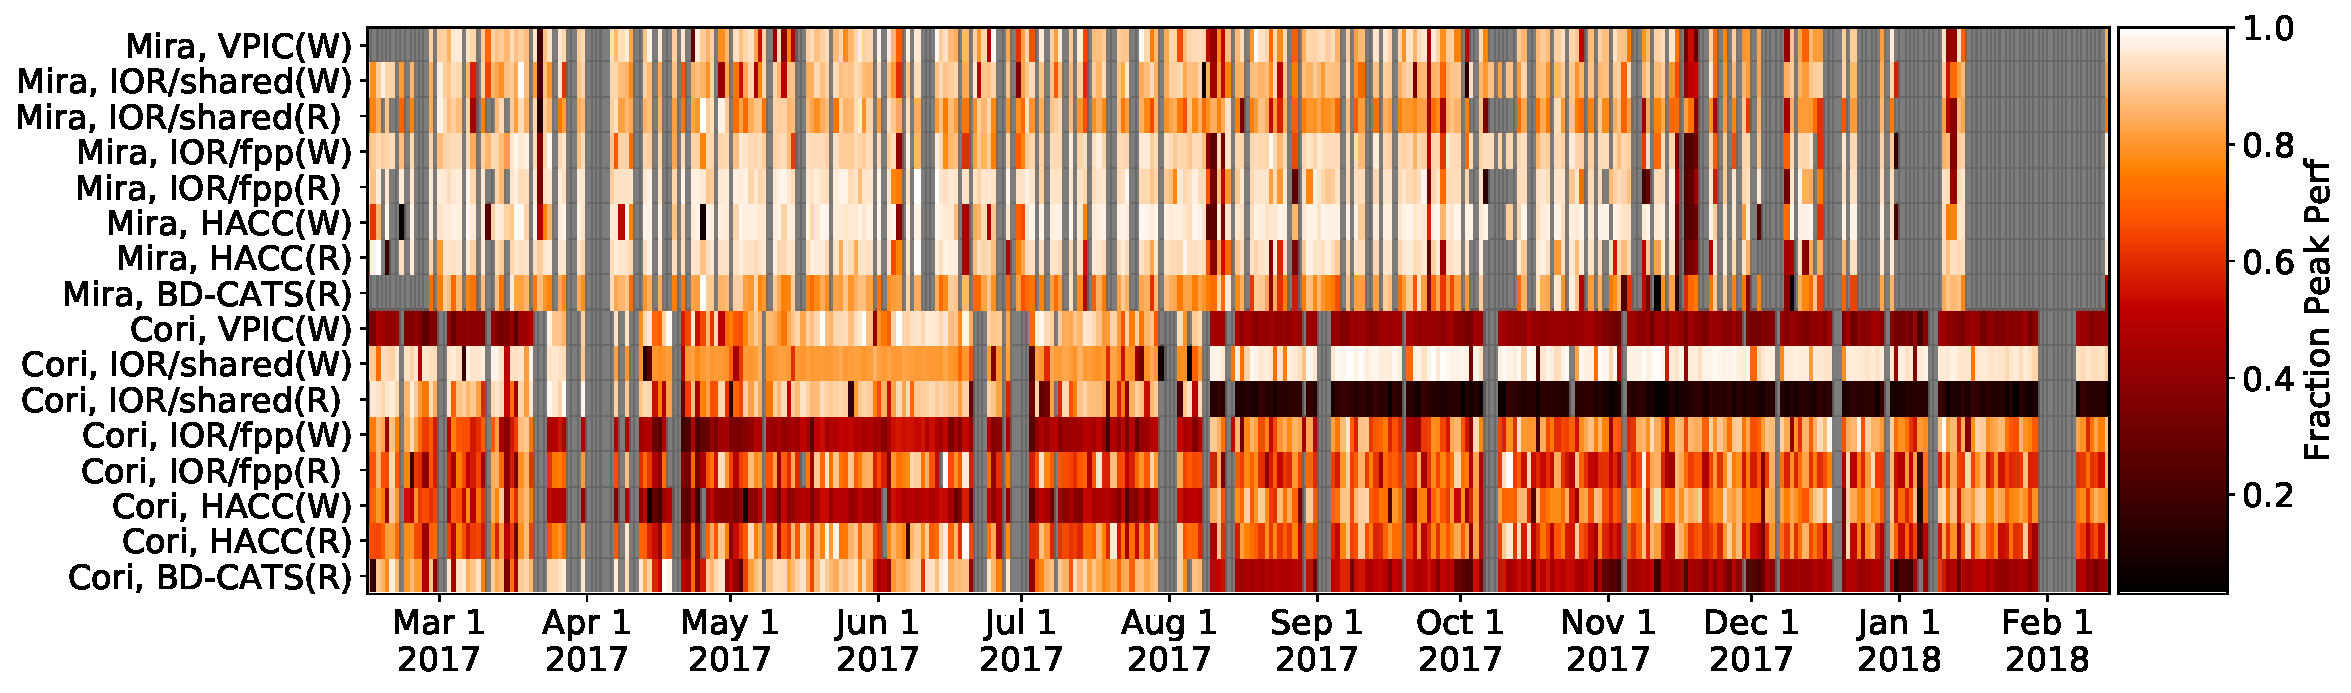
\includegraphics[width=0.90\linewidth]{summary-heatmap}
    \vspace{-.2in}
    \caption{Performance of daily benchmarks normalized to each benchmark's peak observed performance on the specified storage system.  The y-axis labels show combinations of system, I/O motif, and mode (Read/Write).  Grey represents days on which no observations were made.  The two regions highlighted in green boxes are expanded upon in Figure \ref{fig:regions-heatmap}.}
    \label{fig:summary-heatmap}
\end{figure*}

\begin{figure}
    \centering
    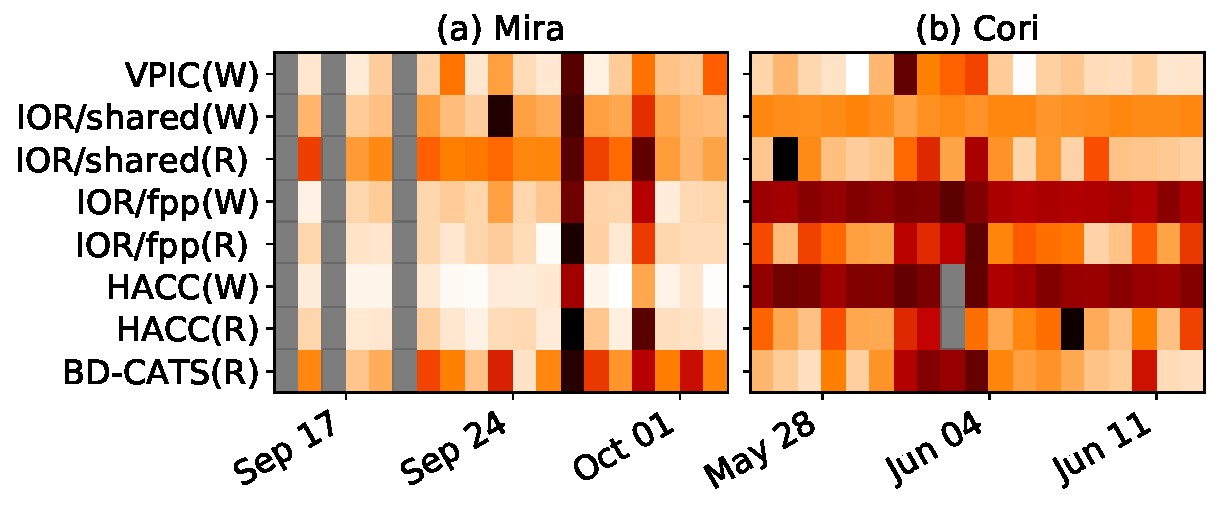
\includegraphics[width=0.90\linewidth]{regions-heatmap}
    \vspace{-.2in}
    \caption{Examples of structure in the fraction of peak performance observations.  Color scale is the same as that in Figure \ref{fig:summary-heatmap}.  In (a), the vertical band on Sept 26 corresponds to a transient system-wide degradation on \mira.  The horizontal bands for the IOR file-per-process write workload (IOR/fpp(W)) and HACC write workload (HACC(W)) in (b) show a sustained performance problem for file-per-process write workloads on \cori.}
    \label{fig:regions-heatmap}
\end{figure}




\subsection{Dataset overview} \label{sec:features/summary}

% \TODO{Things that are important here: behavior over time, grouping data sources in a way that helps understand scope, focusing on fundamental \emph{changes} in performance rather than steady state, everything in one view.}

Absolute I/O performance is influenced by many factors, most notably (a)
application I/O pattern, (b) read/write ratio, and (c) I/O system
architecture~\cite{Lockwood2017, Xie2012}.  This makes it difficult to
reason about performance variation across benchmarks or across platforms,
because each combination is capable of a different baseline performance
level.  We
address this problem by normalizing the
performance of each of the 11,986 observations in terms of its
\emph{fraction of peak performance}.
The fraction of peak performance is defined as the absolute performance (in
bytes/sec) of an observation divided by the maximum absolute performance
observed across all jobs with a common (a), (b), and (c) above.  This
approach allows us to focus on variability for different classes of I/O
workloads rather than their relative performance.

The distribution of the fraction of peak performance measurements for four
of the five systems tested is shown in Fig. \ref{fig:summary-boxplots}.
This figure illustrates that the performance of active I/O performance
probes on production file systems is highly dynamic over the course of a
year.  It does not provide any insight into the temporal nature of the
performance fluctuations, however.

Figure~\ref{fig:summary-heatmap} visualizes the same data in the form of a
heatmap over time.  This shows that performance variation is not randomly
distributed over the year; a key characteristic that is not captured by
time-independent performance distributions.
Several archetypical forms of correlated performance degradation observed in Fig. \ref{fig:summary-heatmap} are highlighted in Fig. \ref{fig:regions-heatmap} and fall into three broad categories of variation:

\begin{enumerate}[leftmargin=*]
\item Dark vertical bands, exemplified in the \mira data in Fig. \ref{fig:regions-heatmap}, represent transient system-wide issues that resulted in a uniform loss of performance for all applications tested that day.
\item Dark horizontal bands, shown in the \cori data, indicate a long-term degradation in performance that disproportionately affects a specific I/O motif.
\item Isolated dark blocks represent individual application runs where performance was poor for a very short period of time within a day.
\end{enumerate}

% - Baseline performance and variability are not constant over time.  Predictive models must therefore adapt over time as well.
The preponderance of these time-dependent phenomena underscore the observation that \textbf{baseline I/O performance and variability are not constant over time}, and
what may qualify as abnormally poor performance during one period of time may be the baseline performance expectation during another.

This has implications for both HPC facility operators and users.  For
facility operators, it indicates that performance anomolies and their root
causes should not be assessed in isolation. By integrating broader spatial and
termporal context into the analysis, facility operators can more accurately
discrinate between applciation problems and environmental factors.
% From Phil: In the prose we can site several predictive model papers (Bing Xie's papers, Sandeep's papers, and others) and point out that the implication is that these models aren't just "set it and forget it."  Not knocking them or even saying they can't do it, but just pointing out it's not covered yet.
For users and application developers, it follows that the accuracy of parameterized I/O performance models~\cite{Xie2012,Madireddy2017} will degrade unless they are reparameterized as the I/O subsystem they model evolves.
Both of these cases justify the need for a systematic approach for identifying different regions of I/O performance to differentiate long-term factors and phenomena from short-term transients.

\subsection{Time-dependent analysis} \label{sec:features/timedependent}

Section~\ref{sec:features/summary} clearly illustrates the presence of
time-varying behavior, but quantitative methods are needed to extract 
actionable insight from these observations.  The main challenge that these
methods face is differentating performance trends from individual short-term
fluctuations in timeseries data.
This problem is not unique to I/O performance or even computer science,
however.  Notably, financial market technical analysis techniques are
routinely used for a similar purpose: attenuating day-to-day volatility in
the price of assets and identifying price movement
trends~\cite{james1968monthly,gunasekarage2001profitability}.  

The most straightforward initial technique to apply from this domain is
the use of Simple Moving Averages (SMAs) over the performance observations.
Given a time window of width $w$, the SMA for performance at time $t$ is the arithmetic mean of the fraction peak performance over ${-0.5w <= t < +0.5w}$.
When chosen to be sufficiently short (${w_{short} \sim O(\textup{days})}$),
the resulting $\textup{SMA}_{short}$ provides a rapid visual means to
identify performance degradation or recovery that lasts for
$O(\textup{days})$.  Multiple SMAs can be plotted simultaneously over the
same data set to differentiate short and long term trends and identify key
crossover points. 

\begin{figure}[t]
    \centering
    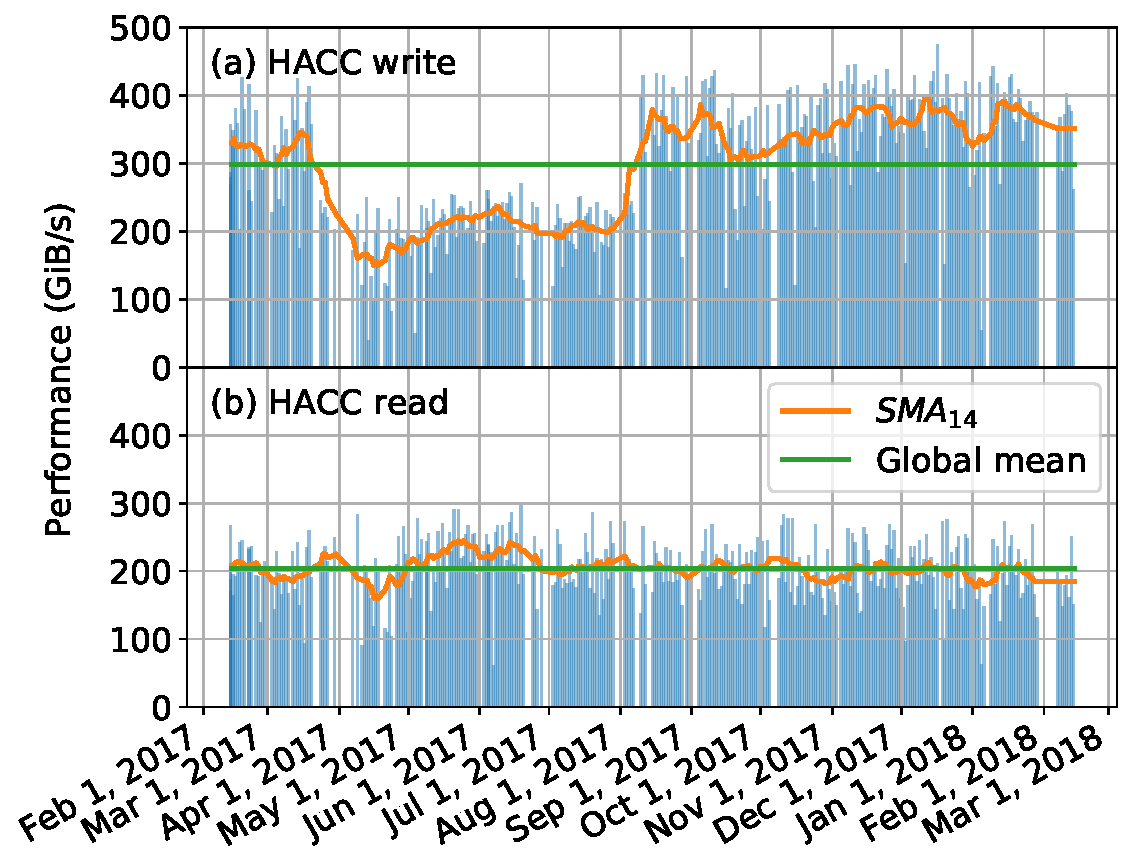
\includegraphics[width=1.0\columnwidth]{longterm-cscratch-hacc}
    \vspace{-.35in}
    \caption{Performance evolution of HACC file-per-process workload on \cori.  Red line is the overall mean (298 GiB/sec write, 204 GiB/sec read) and blue bars are raw performance measurements.}
    \label{fig:timeseries-baseline}
    % source: sc18_segments.ipynb
\end{figure}


An example of an SMA ($w_{short}$ = two weeks) applied to the performance data collected from HACC tests run on \cori is shown in Fig. \ref{fig:timeseries-baseline}.
When contrasted with a time-independent summary statistic such as the overall mean performance of the entire year, the SMA clearly identifies the long period of degraded HACC write performance on \cori that was qualitatively shown in the bottom half of Fig. \ref{fig:summary-heatmap}.
The points at which the SMA rise above or below the global mean performance also provide quantitative measurements of the region of time when an underlying issue manifested;
in Fig. \ref{fig:timeseries-baseline}, these \emph{crossover points} fall on March 24 and August 10.
Cross-referencing these dates with the service history of \cori retrospectively revealed that the beginning and end of this long-term region of divergent performance coincided with major system software upgrades that also happened on March 24 and August 10.

Curiously, the performance of HACC read workload (Figure \ref{fig:timeseries-baseline}b) was unaffected during this time, demonstrating that not all workloads are affected by long-term variation equally.
This asymmetry, in combination with the bounding dates of this divergent region, allowed us to trace this specific issue to unintentional behavior introduced (and later fixed) in the Lustre software running on \cori during the system upgrades.
Although this particular case of long-term performance divergence was caused by an unexpected bug in system software, the reality of most production storage systems is that they are regularly patched and upgraded.
At minimum, the security requirements of the centers which run them drive system updates, and as exemplified by the widely publicized Spectre and Meltdown patches, such updates can have non-trivial effects on certain types of I/O.
Thus, \textbf{administrative activities such as maintenance patches and
software updates are a significant source of time-dependent, long term performance
variation.}  This must be accounted for in both retrospective performance
analysis and forward looking performance modeling parameterization.  The
ramifications I/O research practitioners is that \textbf{holistic I/O monitoring
should incorporate environmental provinence
information, such as kernel, operating system, and file
system version, to aid in correlation.}

\subsection{Regions of interest} \label{sec:features/partitioning}

We can generalize the analysis technique from
Section~\ref{sec:features/timedependent} 
by superimposing a second SMA ($\textup{SMA}_{long}$) with a longer window (${w_{long} \sim O(\textup{weeks})}$) on top of $\textup{SMA}_{short}$ (which captures variations ${O(\textup{days})}$).
Doing so allows us to examine short-term performance variations (e.g., a
period of sustained bandwidth contention) in the context of longer-term
trends (e.g., in the presence of a file system software regression).  Once a
region of interest has been defined, we can then constrain more detailed
analysis techniques to that region to determine its cause.
The points at which $\textup{SMA}_{short}$ intersects $\textup{SMA}_{long}$, termed \emph{crossover points}, conveniently establish the boundaries of regions where short-term performance has diverged from longer-term performance and anomalous performance is prevailing.
We therefore introduce the notion of \emph{divergence regions} which are the periods of time bounded by two crossover points and capture correlated performance.
Fig. \ref{fig:mira-regions-overview} depicts how these concepts are combined in a subset of the data collected.

For the remainder of this study, we apply the concept of \emph{divergence regions}, bounded by the crossovers between $\textup{SMA}_{short}$ and $\textup{SMA}_{long}$, to systematically identify and characterize periods in time where anomalous performance was observed by the active I/O probes running across all of the test systems.
We define $\textup{SMA}_{short}$ to have $w_{short} = 2 \textup{ weeks}$ as in \ref{sec:features/timedependent} and $\textup{SMA}_{long}$ to have $w_{long} = 7 \textup{ weeks}$.
$w$ was chosen to be a multiple of seven days to align with one
week and ensure that weekends and weekdays were equally represented both SMA
calculations. (The HPC resources e $w_{long}$ was set to 7 weeks to span multiple $w_{short}$
regions and at least one month boundary.  In our experience, the analysis
presented in this work was insensitive to changes of $\pm 1 \textup{ week}$.

\TODO{Possibly redundant, but reading to this point without having read the next section, it would be helpful to have the top half of Figure 5 here to illustrate a shaded region bounded by crossover points.  Maybe split it, or repeat it?
\\
gkl-hopefully Fig. \ref{fig:mira-regions-overview} addresses this}

In general we find that \textbf{financial market technical
analysis techniques can be adapted to
timeseries I/O performance data to attenuate noise and identify underlying trends.}
In the context of financial markets, SMAs (and other more
sophisticated related techniques) are used for predictive purposes to time
the execution of market trades.  In this context we are not applying them to
the task of predicting performance, but rather to identify regions of
interest in behavior that has already been recorded.

\begin{figure}
    \centering
    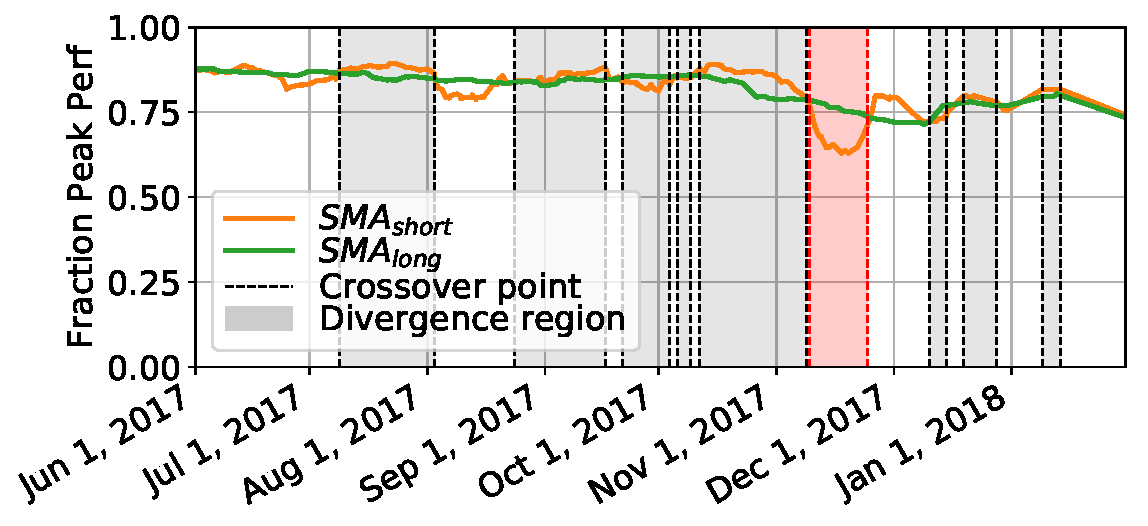
\includegraphics[width=1.0\columnwidth]{mira-regions-overview}
    \vspace{-.15in}
    \caption{Schematic depicting the relationship between SMAs, crossover points, and divergence regions on \mira.
    Both white and grey regions between crossovers are divergence regions, but only a subset of divergence regions are shaded for clarity.
    The significance of the divergence region highlighted in red is discussed in Section \ref{sec:results/correlate-mira}.}
    \label{fig:mira-regions-overview}
    % source: sc18_region-correlation.ipynb
\end{figure}


\section{Investigating Trends}\label{sec:results}

SMA crossover-based partitioning of performance observations provides
a systematic method for grouping time-correlated performance events.
Once a divergence region (i.e., a performance trend) has been identified,
more focused statistical analyses can then be applied within the region
to gain insight into the factors that contributed to that trend.  Examples of
contributing factors may include utilization, system health, and component performance.
In the following analyses, we separate our 11,986 performance observations into sets of observations that all ran on the same test platform (as described in Table \ref{tab:platform-descriptions}) to characterize the factors that contribute to time-dependent performance variation across different file systems and architectures.

\subsection{Correlative analysis} \label{sec:results/correlate-mira}

\begin{figure}
    \centering
    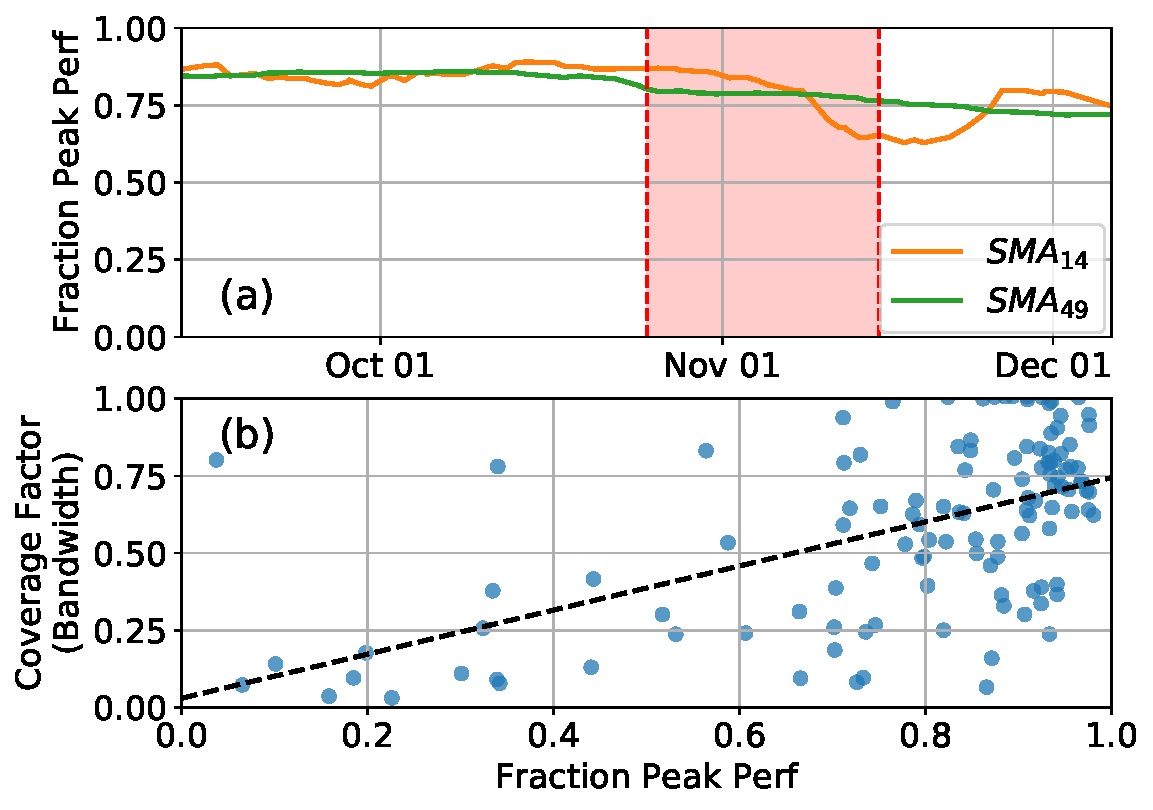
\includegraphics[width=1.0\columnwidth]{mira-correlation-region}
    \vspace{-.35in}
    \caption{Correlation between performance and $CF_{bw}$ in a divergence region on \mira for all I/O motifs combined.
    (a) highlights the divergence region of interest and corresponds to the same highlighted region shown in Fig. \ref{fig:mira-regions-overview}. (b) shows the correlation between performance and $CF_{bw}$ in that region.
    Correlation coefficient is $0.507$ and p-value is ${8.71 \times 10^{-9}}$; dashed line in (b) is a linear fit with slope $0.503$ drawn for visual aid.}
    \label{fig:mira-correlation-region}
    % source: sc18_region-correlation.ipynb
\end{figure}

% Bandwidth, IOPS, and metadata contention are confidently correlated with I/O performance at both long. 

\TODO{add a footnote explaining p-value}
We begin our correlative analysis by partitioning a year-long data set into
divergence regions using the method described in
Section~\ref{sec:features/partitioning}.  Using observations from \mira
\mirafsone as an example, we set ${w_{short} = \textup{two weeks}}$ and ${w_{long}
= \textup{seven weeks}}$ to identify divergence regions, and then discard any
regions with fewer than three data points.  Regions with few data points are discarded
for two reasons: (a) intuitively, very short divergence regions occur
when $\textup{SMA}_{short} \approx \textup{SMA}_{long}$ and there is
minimal long-term variation, and (b) statistically, it is impossible
to assert the statistical significance of a correlation with fewer than
three data points.  This yields 32 divergence regions.

We then apply Pearson correlation~\cite{Falk97manyfaces} to the feature vectors within each divergence region to identify the factors that correlate with its
performance trend.
The result of this process is a new feature vector for each divergence region which contains the correlation coefficients between the fraction of peak performance and every other attribute across all observations in that region.
We then use the p-value of each correlation coefficient\footnote{
The p-value of a correlation coefficient is the probability of observing data that would show the same correlation coefficient in the absence of any real relationship between the underlying metrics.
A low p-value indicates that it is extremely unlikely that the calculated correlation coefficient would be observed if the metrics being compared had no real correlation.
As such, p-values represent the statistical significance of a statistical measurement.}
to further downselect the total set of regions to those with extremely high significance
($\textup{p-value} < {1.0 \times 10^{-5}}$).
This threshold yields a total of nine relevant divergence regions on \mira \mirafsone which are all depicted as shaded extents in Figure \ref{fig:mira-regions-overview}.
Each of these nine regions exhibits at least moderate correlation ($R$) ranging from 0.507 to 0.884 with the bandwidth coverage factor feature.

\TODO{I'm not sure I understand why we're aggregating divergence regions from different motifs here, since everywhere else our analysis is applied to these independently. For one, different motifs could have different trend regions by definition. If the results hold over just one motif, maybe just use those, or something? -SS}
Fig.~\ref{fig:mira-correlation-region} illustrates the correlation between bandwidth coverage factor and fraction peak performance for a particular divergence region in November 2017 on \mira \mirafsone.
This example exhibits the lowest correlation ($R = 0.507$) with bandwidth coverage factor of any of the selected regions, and the scatter plot of performance results shows why:
this region contains a cluster of poorly performing probes (${0.2 < \textup{fraction peak perf} < 0.4}$) that ran with a relatively high bandwidth coverage factor.
This region is also the single largest divergence region observed on \mira; a difference of over 20\% between $\textup{SMA}_{short}$ and $\textup{SMA}_{long}$ was observed during this time.
This divergence region example highlights the importance of not just identifying regions and calculating correlations, but identifying cases in which the analysis indicates the presence of an unknown factor that is not adequately captured by the instrumentation framework.

Despite the unusual region shown in Fig. \ref{fig:mira-correlation-region},
however, these data indicate that the time-dependent performance divergences observed on \mira show either moderate or strong correlation with bandwidth contention.
Additionally, this correlation with performance degradation occurs across
\emph{all} I/O motifs (similar to Figure \ref{fig:regions-heatmap}a) which
distinguishes it from the motif-specific case discussed in Section
\ref{sec:features/timedependent}.  

When the same Pearson correlation is calculated across the entire collection
of \mira \mirafsone data in the absence of partitioning, the correlation with bandwidth coverage factor
yields an overall result of $R = 0.483$ and $\textup{p-value} =
2.25\times 10^{-88}$.  \textbf{Thus, significantly stronger
correlations can be found by focusing analysis on algorithmically identified regions of
interest in the data.}

% \TODO{We could use a plot for comparison if we have a lot of free time to
% kill.  I don't think it is critical though.}

\subsection{Survey of divergence regions} \label{sec:results/correlate-all}

% - Bandwidth, IOPS, and metadata contention are confidently correlated with I/O performance at both long. 



\begin{figure}
    \centering
    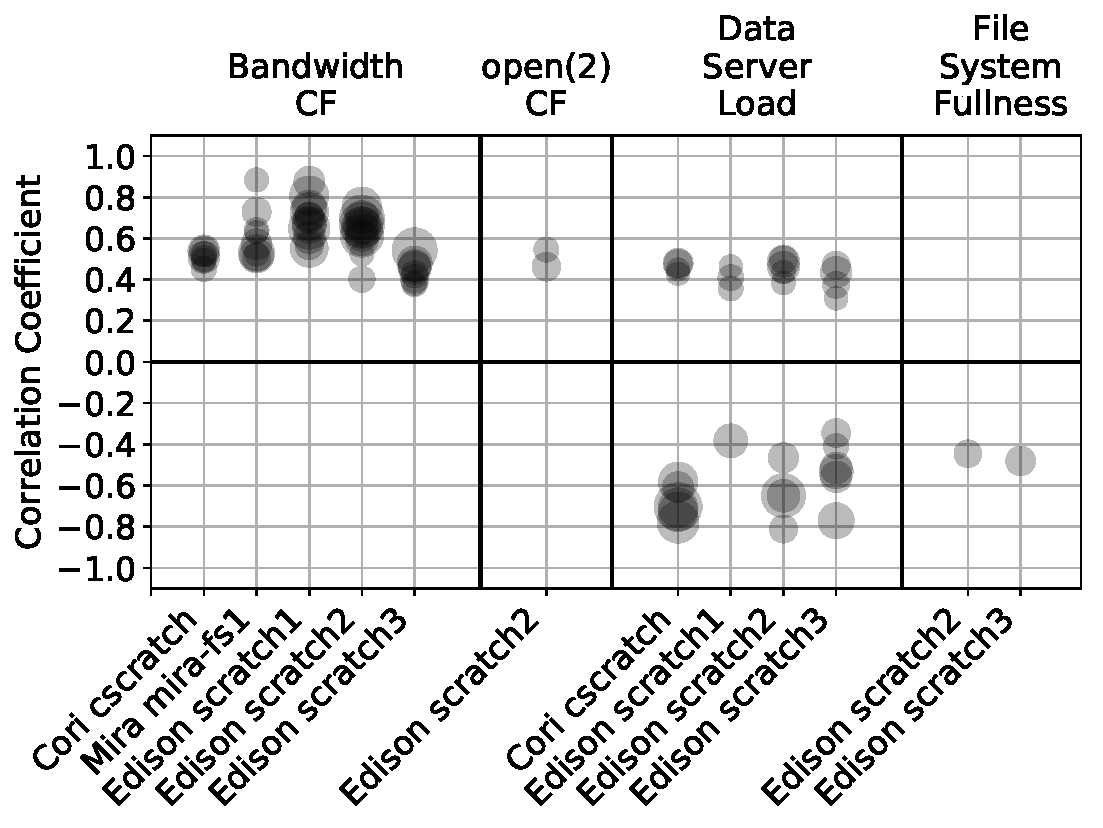
\includegraphics[width=1.0\columnwidth]{trend-correlations}
    \vspace{-.35in}
    \caption{Correlations discovered between fraction peak performance and all other attributes measured during job execution.
    Each circle represents the correlation coefficient over a single trend region, and its diameter is proportional to $-\log_{10}(\textup{p-value}$).
    CF denotes coverage factor.}
    \label{fig:trend-correlations}
    % source: sc18_region-correlation-all.ipynb
\end{figure}



Next we apply the same correlation analysis to the other test platforms in our study, again only keeping correlations with an extremely high significance ($\textup{p-value} < {1.0 \times 10^{-5}}$), and the results of this analysis are shown in Fig. \ref{fig:trend-correlations}.
As was found with Mira in Section \ref{sec:results/correlate-mira}, there is moderate to strong correlation between I/O performance and the bandwidth coverage factor on the Lustre file systems of \cori and \edison.
Although bandwidth contention resulting in performance loss is intuitive at the scale of a single performance transient, the fact that these correlations were found over longer-term divergence regions indicates that \textbf{bandwidth contention from \emph{sustained workloads} often accompanies sustained performance losses}.
This is particularly relevant to the increasing fraction of experimental and observational data that is being processed on modern HPC platforms; as the volume of data being continually streamed from large-scale scientific instruments increases, the effects of sustained bandwidth contention are likely to become increasingly prominent.

% - The sign and magnitude of the correlations changes over time.

\begin{figure}
    \centering
    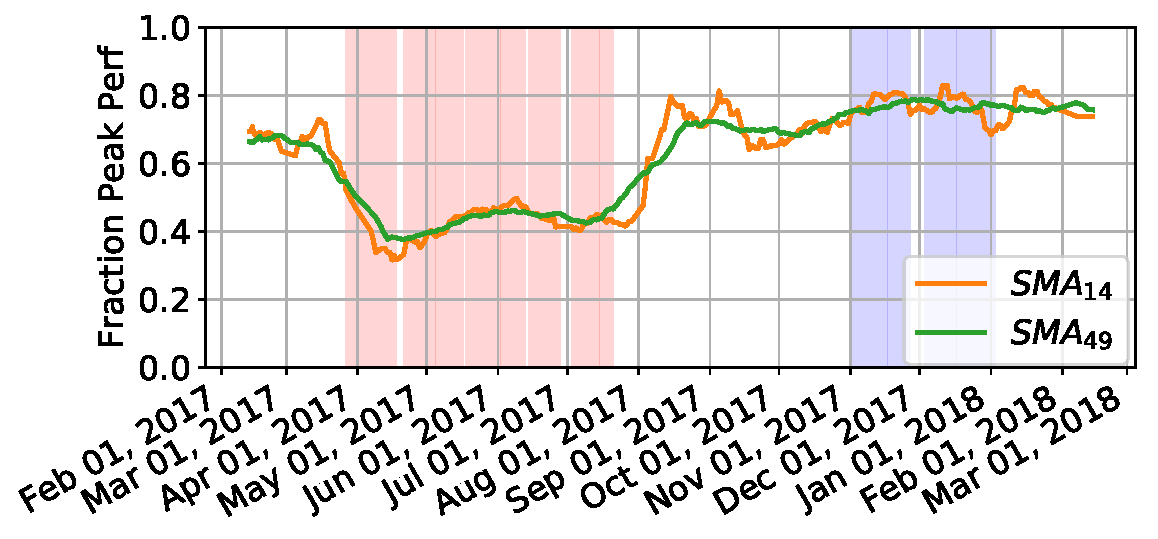
\includegraphics[width=1.0\columnwidth]{cscratch-bimodal-fsaveosscpu}
    \vspace{-.35in}
    \caption{Regions of negative correlation (red) and positive correlation (blue) between fraction peak performance and data server load during trend regions identified on \cori.
    SMAs for \cori's HACC write workload also shown to illustrate the coincidence of a long-term performance issue with the direction of correlation.}
    \label{fig:cscratch-bimodal-fsaveosscpu}
    % source: sc18_region-correlation-all.ipynb
\end{figure}


Another noteworthy feature that this method reveals is the bimodality of correlation between performance and the CPU load of the file system data servers (``Data Server Load'' in Fig. \ref{fig:trend-correlations}) on the Lustre-based test platforms.
A time-resolved view of the regions where performance correlates with data server CPU loads (Fig. \ref{fig:cscratch-bimodal-fsaveosscpu}) reveals that the bimodality of the correlation matches the biomodality observed in the HACC write workload on the affected storage systems.
During the long-term performance regression discussed in Section \ref{sec:features/timedependent}, high CPU load on the Lustre OSSs coincided with low performance of the I/O performance probes.
As soon as performance was restored on August 10, the relationship reversed, and high CPU load was observed favorably with respect to performance.

The positive correlation between performance and CPU load is consistent with the data servers using CPUs primarily to service incoming I/O requests, whereas the negative correlation indicates that another CPU load (as may be caused by an algorithmic bug) was present and competed with the data servers' ability to use CPU to service those same requests.
From this, we conclude that not only does baseline I/O performance vary with time, but \textbf{the nature and magnitude of how different attributes correlate with I/O performance also change over time}.
Had this correlation analysis been performed without partitioning over divergence regions, the regions of positive and negative correlation would have obfuscated each other in the net result.

The remaining two attributes that were found to correlate with performance
are file system fullness and \texttt{open(2)} coverage factor (a
measure of metadata resource contention).  The two instances of file
system fullness correlating negatively with performance are clear
and can be corroborated with independent observations from facilities
staff.  These two regions encapsulate periods when their respective
file systems approached 90\% fullness for a period of several days.
The observed loss of performance is consistent with Lustre's known
susceptibility to significant performance degradation as OSTs approach
90\% fullness~\cite{oral2014best,Lockwood2017}.

The correlation with
\texttt{open(2)} coverage factor is intuitive because this metric acts as a
proxy for metadata contention.  
One of these divergence regions was found to overlap with an unusually extensive, long-running multi-day purge of the \edison \scratchtwo file system.
However, it is unclear at this time what caused the other correlated divergence region.
% The above statement is not very satisfying, but we don't have time to do more detailed analysis.  The regions are:
% coverage_factor_opens 2017-03-29 19:11:51 - 2017-04-15 19:13:37 (71 points)
% coverage_factor_opens 2017-11-26 18:26:41 - 2017-12-13 20:03:11 (141 points)


\subsection{Transient performance loss} \label{sec:results/shortterm}

\begin{figure}

    \centering
    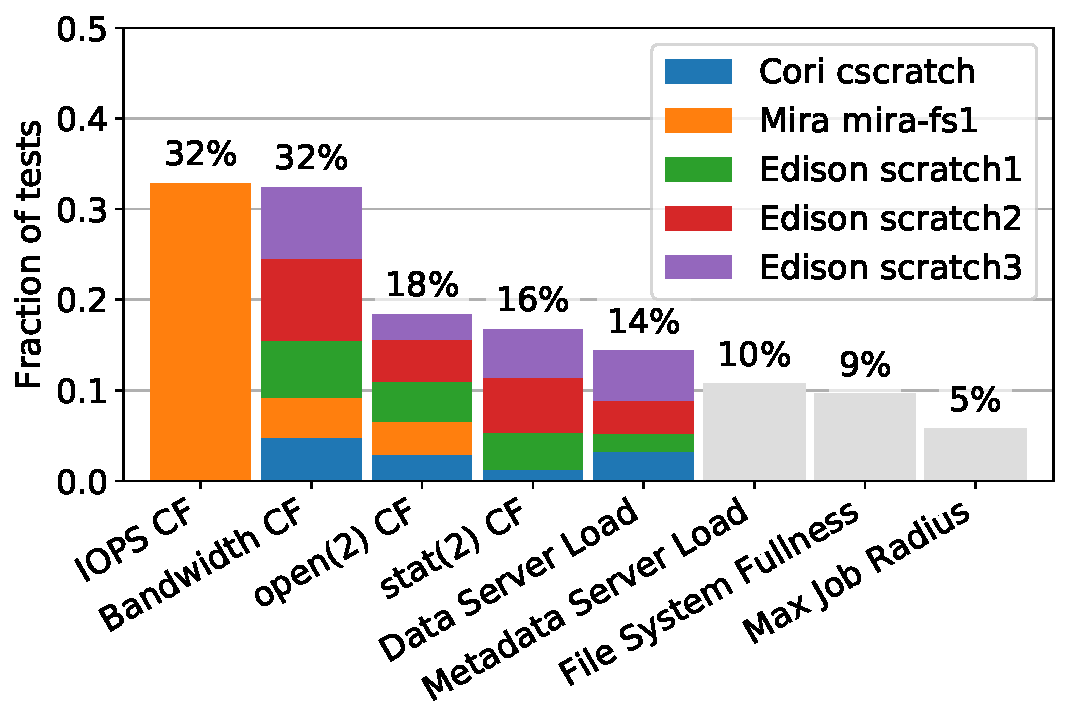
\includegraphics[width=1.0\columnwidth]{contributors-bad-by-system-grey}
    \vspace{-.35in}
    \caption{Attributes that correlated with poor I/O performance across all file systems and benchmarks tested normalized to the number of probes during which each attribute was measured.
    \mira was the only system for which IOPS coverage factor was measured.
    Greyed bars are attributes whose aggregate contributions were not statistically significant.
    Percentages do not add up to 100\% because multiple attributes are often classified as contributors for a single anomalous observation.
    }
    \label{fig:contributors-bad-by-system}
    % source: sc18_umamify-all.ipynb
\end{figure}

In addition to characterizing long-term performance issues, it is also advantageous to determine the reasons why I/O performance is severely degraded for one and only one day in an otherwise unremarkable period of time.
Such performance losses, exemplified as isolated dark blocks in Fig. \ref{fig:regions-heatmap}, may only be observed in one of the I/O performance probes issued on that day, suggesting a very short-lived issue that disappeared over the course of one or two of the eight daily probes.
The lack of a consistent performance trend surrounding these transients makes them difficult to correlate with other metrics as was done in the previous section, necessitating a different approach to characterizing them.

To address this need, we apply the same strategy of partitioning performance observations into divergence regions and then performing statistical analysis within each region.
To identify individual performance anomalies in a divergence region and classify the factors which contributed to them, we apply the following binary classification method:
\TODO{Are we sure we only want to determine one and only one anomalous observation in each divergence region? -SS}

\begin{enumerate}[leftmargin=*]

\item We examine the feature vector for every observation in the divergence region, and for each attribute $a$, determine the observation where that attribute's measured value was at its lowest, $\min(a)$.

\item We then define the \emph{anomalous observation} for the divergence region as the observation whose feature vector contains $\min(a)$ for fraction peak performance.
As divergence regions contain observations of similar performance by definition, this anomalous observation is truly anomalous-- it is differentiated from the long-term performance trends described in Sec.~\ref{sec:features} as well as the ones within its own divergence region.

\item Finally, we determine which other $\min(a)$ values also fall in this anomalous observation's feature vector and classify those attributes as contributors to the anomalous observation's performance.

\end{enumerate}

Qualitatively, this process codifies the conjecture that if I/O performance is anomalous on a specific day, the other measured attributes which were also anomalous at that time are what contributed to that behavior.
Quantitatively, this simple classification scheme allows us to identify relationships and define the statistical significance of each classification for individual anomalous observations using p-values\footnote{
The p-value is the probability of making a positive classification in the absence of an underlying relationship or, equivalently, the probability of positively classifying a random value.
Since there is only one $\min(a)$ in each region of $N$ observations, the p-value for our classifications is thus $\frac{1}{N}.$}.

The result of this process is zero or more attributes being positively classified as contributors to anomalous performance.
For example, if the lowest values of the bandwidth coverage factor and IOPS coverage factor attributes occur in the same feature vector as the lowest value for performance, we classify both bandwidth and IOPS coverage factors as contributors to that anomalous observation's performance.

To apply this method, we first group observations into sets of data by the test platform on which they ran as was done in Section \ref{sec:results/correlate-mira}.
These sets are then further subdivided according to I/O motif and read/write mode of the probe to classify anomalies at full temporal resolution and motif-level granularity.
The net result are $5 \times 4 \times 2 = 40$ sets of data, each representing a unique combination of test platform ($5 \times$, as listed in Table \ref{tab:platform-descriptions}), I/O motif ($4 \times$, per Table \ref{tab:benchmark-motifs}), and whether the probe was reading or writing ($2 \times$).
Schematically, each horizontal row in Figure \ref{fig:summary-heatmap} represents a single set.
For each set of observations, SMAs are calculated, crossover points are defined, and the set is partitioned into a set of divergence regions.

This partitioning results in 1,146 divergence regions across 40 sets of observations, each containing one anomalous observation.
For each divergence region, we then apply the aforementioned binary classification to generate positive classifications of attributes that affected performance and their p-values.
We discard all statistically insignificant classifications ($\textup{p-value} > 0.10$) to eliminate divergence regions that are too small to make any meaningful classifications, positive or negative.
The final products are 490 anomalous observations, 410 of which have at least one attribute positively classified as a contributor.

As described in Section \ref{sec:methods/tokio}, not every observation's feature vector has every feature defined.
So as not to bias our results away from those attributes that were only measured for a subset of observations (e.g., IOPS coverage factor was only collected on \mira), we calculate the frequency of each attribute as the ratio of observations where it was defined \emph{and} classified to the number of observations where it was defined.
The result of this aggregate frequency summary is shown in Figure \ref{fig:contributors-bad-by-system}.
\TODO{Glenn to clean up above paragraph}

As with the longer-term performance divergence characterized in Section \ref{sec:results/correlate-all}, high contention for bandwidth is found to also coincide with short-term performance transients.
However, contention for IOPS is also positively classified in a significant fraction of anomalous observations despite it not arising as a factor in longer-term performance divergence.
This contrast demonstrates that IOPS contention only becomes a statistically significant attribute related to performance degradation in short-term transients, and there are no sustained periods of high IOPS on \mirafsone.
This also distinguishes this utility of this transient classification from
the longer-term correlative analysis.
% Intuitively this result makes sense, as a job running on the machine performing I/O only places load on the metadata server during short duration events (eg. file open/close), whereas the load when the data is being read or written is likely to occur over much longer time periods.
% Intuitively, this result makes sense; a job performing I/O nominally places load on the metadata server only at the start and end of of reading and writing, while the process of reading and writing occurs over much longer time periods.
% \TODO{gkl: Phil/Shane, please review above line with your I/O expert hat on}

We also observe the coincidence of anomalous jobs and anomalous metadata coverage factor and CPU load on
data servers to a less significant degree.  This is
consistent with the moderate correlations shown in
Figure~\ref{fig:trend-correlations}.
Unlike the correlative analysis, however, metadata contention was found to impact individual jobs on every test platform and occurred at much higher frequency.
These findings indicate that metadata contention is much more likely to coincide with transient performance loss than a long-term and sustained divergence of performance.

In general, the contrast in correlations between transient events and
long-term trends shows that \textbf{the attributes that correlate with transient
performance problems (IOPS and
  metadata contention) often differ from those that correlate with
    long-term performance problems (bandwidth contention).} These are two distinct forms of performance variation that
require unique investigation techniques.

\TODO{Simplify our motivation for doing this bimodal stuff--we saw some metrics that correlated infrequently.  Are these statistically significant?
\\
"frequency of attributes" should go away--we're talking about how often $a$ pops up in "instance of slowdowns"
}
Metadata server CPU load, file system fullness, and maximum job radius were also classified in some anomalous observations.
However, the low number of anomalous observations in which they appeared calls into question the statistical significance of these three findings.
To address this, we calculate the p-values, or the probability of observing the same number of classifications in the absence of a true underlying relationship, for each metric\footnote{
To calculate these p-values, we use one-tailed binomial tests using the number of positive classifications observed for each metric.
The fact that our dataset was filtered to only include regions with ${\textup{p-value} < 0.10}$ also establishes 0.10 as the most conservative value for the binomial test probability.}.

The result of these significance tests reveal that the number of times metadata server load, file system fullness, and maximum job radius were classified is statistically insignificant.
Whereas the leftmost five attributes in Fig. \ref{fig:contributors-bad-by-system} all have p-values of ${5 \times 10^{-5}}$ or lower, the insignificant metrics' are 0.15 or higher.
Qualitatively, these negative findings are not unreasonable; for example, file system fullness is most often a degenerative, long-term health problem as was identified in Section \ref{sec:results/correlate-all} and prior work~\cite{oral2014best,Lockwood2017}.

The classification process and analysis described here demonstrates that it is possible to apply statistical analysis to fine-grained divergence regions and still obtain statistically significant insight into the causes of transient performance degradation.
While we chose a very simple binary classification criteria based on $\min{a}$, this process could be applied using any classification methodology that identifies relationships between feature vectors in a divergence region and quantifies the associated statistical significance.


\endinput

% NJW - this sentence adds too much complexity to end the section with
% 
%%%For example, classifying attributes based on quartiles rather than minima would be feasible with more coarse-grained divergence regions to offset the decrease in significance inherent in the selection criteria.

\subsection {Discussion}
\label{sec:results/discussion}

\TODO{This is where interesting dribs and drabs are winding up.  Do we carve out a separate section about this stuff, or just drop it?}

Our choice of averaging $\textup{SMA}_{short}$ over ${-0.5w_{short} <= t < +0.5w_{short}}$ makes it insensitive to choice of $w_{short}$.
For the analysis in Section \ref{sec:features/timedependent} changing $\textup{SMA}_{short}$ from $\textup{w}_{14}$ to both $\textup{w}_{7}$ and $\textup{w}_{28}$ resulted in no change to the dates bounding the 139-day divergence region.
The principal effect of changing $\textup{w}_{short}$ is the number of short regions that arise from the higher-frequency oscillations of $\textup{SMA}_{short}$ around $\textup{SMA}_{long}$.

\TODO{This is where a discussion about performance models having to account for long-term changes to baseline performance should go.  That doesn't seem to fit well into the rest of the narrative though.}

We found the exact choice of $w_{short}$ and $w_{long}$ to be somewhat arbitrary; adjusting these values by as much as $\pm 50\%$ did not affect the identification of the most significant events presented here.
In addition, a specific choice of $w$ does not preclude analyzing events longer or shorter than $w$, and we demonstrate methods to address this in Sections XYZ.

Although SMA crossover points are also applied in market analysis for detecting trends in prices and predicting when to buy or sell an asset based on the direction of the crossover~\cite{brock1992simple}.
However, the predictive value of SMA crossovers is a source of controversy even in the financial community, and thus, we focus here solely on using them as tools for detecting trends and partitioning divergent regions in historical datasets.

Financial market analysis techniques can be used to detect underlying trends within noisy I/O performance data.


\section{Findings and Implications for State of the Practice}
\label{sec:findings}

% The key findings of this study have been presented thus far in an
% order dictated by a hierarchical, data-driven investigation of our
% I/O performance data set.  We can now revisit those findings, however,
% and reclassify them according to their impact the state of
% the practice.

This study has revealed a number of novel insights into the nature of I/O performance using holistic I/O analysis and active I/O performance probes.
In addition, our findings have significance beyond the scope of the specific systems evaluated, and they collectively constitute an advancement to the greater state of the practice.
In this section, we revisit the most significant outcomes and provide corollaries that will improve our ability to contextualize, quantify, and analyze I/O performance variability on large-scale storage systems.

\subsection{Understanding large-scale storage system behavior}

The following findings serve to refine our understanding of how large-scale storage
systems behave at a high level: 

\begin{itemize}[leftmargin=*]

\item \textbf{Baseline I/O performance and variability are not constant over
time:} This observation has direct implications for our specifications and
expectations of system performance.  It is unrealistic to assume that
benchmarks performed upon system delivery will accurately represent
performance over time, and performance expectations must be recalibrated as storage systems age.

\item \textbf{Attributes that correlate with transient performance problems  often differ from those that correlate with
long-term performance problems:}  I/O-intensive workloads in HPC
are widely known to be unusually bursty compared to other I/O-intensive markets, but this finding reveals that some aspects of HPC I/O workloads (such as IOPS
and metadata contention) are burstier than others (such as bandwidth contention).  Performance degradation that results from metadata or IOPS contention is unlikely to persist for days or weeks, while bandwidth contention can result in variation at all time scales.

\end{itemize}


\subsection{Improving monitoring and telemetric coverage}

The following findings motivate further advances in how large-scale storage systems are monitored and what data sources are required:

% \TODO{\textbf{where does this go?  tempted to drop it since it's specific to our results, not the state of the practice}
% Furthermore, 16\% of the transient I/O performance issues defied classification using our binary classification method.
% This indicates that we are still missing telemetry from important components of the I/O subsystem that contribute to performance variation.}

\begin{itemize}[leftmargin=*]

\item \textbf{Administrative activities such as maintenance patches and
software updates are a significant source of time-dependent, long term
performance variation}: HPC systems are complex, and their upgrades may be
dictated by a variety of external factors including maintenance schedules,
vendor release cycles, and security concerns.  Because of this, it may not be
possible to capture explicit before and after measurements as part of the
upgrade process.  Continuous monitoring and active probing of performance
can mitigate this problem by making such measurements a routine procedure regardless of upgrade
schedule, much in the same way that continuous integration testing is used
to automatically monitor software development processes.

\item \textbf{Holistic I/O monitoring should incorporate environmental
provenance information, such as kernel, operating system, and file system
versions, to aid in correlation}: 
This is an obvious finding in retrospect, but is not widely taken into
account in current instrumentation tools.  Tools such as Darshan and
LMT should capture sufficient environmental information 
alongside conventional performance measurements to
simplify the task of identifying performance losses due to environmental changes.

\item \textbf{Bandwidth contention from sustained, I/O-intensive workloads often accompanies
sustained performance losses}: The impact of bandwidth contention on I/O
performance is widely supported in the literature, but this study demonstrates
time-dependent behavior not previously acknowledged. Specifically, detrimental contention
can occur over time spans lasting several weeks (e.g., aggregate
workload due to project allocation timing) and may be driven by factors 
not captured by conventional HPC monitoring (e.g., wide area transfers or 
archival traffic).  This calls for a broadening of the definition of
``holistic I/O characterization'' to include not just the full HPC I/O
stack, but also the auxiliary resources that utilize the storage system.

\end{itemize}


\subsection{Analyzing evolving storage systems}

Finally, the following findings highlight ways in which the accuracy and significance of 
I/O analysis and modeling methodologies can be improved:

\begin{itemize}[leftmargin=*]

\item \textbf{Financial market technical analysis techniques can be adapted
to I/O performance time series data to attenuate noise and identify
underlying trends}: Processing a large, continuously expanding, and noisy
time series data set is a daunting task, but one that is not unique to I/O
performance characterization.  We found similarities
between our data set and financial market data that enabled straightforward
adaptation of known techniques and terminology.  More advanced financial
market technical analysis strategies or strategies from other similar fields would likely be even more effective.

\item \textbf{Significantly stronger correlations can be found by focusing
analysis on algorithmically identified regions of interest in the data}:
There is considerable temptation with the emergence of machine learning and
deep learning to apply unguided techniques to a large data set in a bid to
extract meaning from it. From a practical point of view, however, a systems
practitioner will gain more benefit from targeted analysis of relevant regions of
interest.  The region identification method need not depend on SMAs, and alternative
approaches for both partitioning time series data and classifying the
measurements within regions can be easily improved with more sophisticated methods.
%Our hope is that the simple statistical methods presented here will advance
%the state of the practice across the HPC community by encouraging
%straightforward methods that improve the efficacy of quantitative I/O analysis.

\item \textbf{The nature and magnitude of how different attributes correlate
with I/O performance also change over time:}  This observation has critical
ramifications for developing and applying I/O performance models.  Models developed from a training set without temporal context
will produce incorrect predictions, even on the same target system, if
external factors have caused the performance of that system to evolve over
time. For example, we demonstrated that high CPU load can correlate with favorable performance under healthy file system conditions, and it can coincide with unfavorable performance when non-I/O workloads are impacting storage servers.

\end{itemize}

\section{Conclusion} \label{sec:conclusions}

Our study of a year in the life of a parallel file system provided a
variety of insights into performance variation on production systems,
including both long-term trends and transient anomalies.  These insights,
and the methods that we used to derive them, have implications for
instrumentation methods, administrative expectations, and analysis
techniques. Some of the recommendations in these findings can be acted on
now by broadening the scope of instrumentation or enhancing analysis tools based on observations in this paper.
Others more fundamentally motivate the need for ``live'' analysis of
production systems so that the lessons learned here (especially those
related to dynamic, time-dependent behavior) can be more generally extracted
at any time from a running system to produce actionable feedback.

Near term future work calls for the development of additional \tokio
connectors to incorporate additional storage resources such as burst
bufferss.
In the long term, we plan to develop methods to systematically classify the
similarity of different regions from one another and enable the
determination of broad classes of performance regions.
We will also use the measured data as input for simulation frameworks to
enable the design of potential new file system features or policies that may
reduce the amount of I/O performance variation seen in production. 
\endinput

\begin{enumerate}

\TODO{these lack "implications for state of the practice"; need to take these up a level.  if we were selling this process to another center, what would they need to take from this study?}

\item \textbf{Baseline performance and performance variation changes over time.}
We have shown that the baseline peak performance for a given I/O motif on a file systems can change over time as a result of factors such as system software updates and sustained workloads motivated by external factors such as end of allocation year.
\TODO{1. you can't just measure performance on day 1}

\item \textbf{The magnitude and sign of correlation between performance and other measured metrics also varies over time.} 
We demonstrated that high CPU load can correlate with favorable performance under healthy file system conditions, and it can coincide with unfavorable performance when non-I/O workloads are impacting storage servers.
\TODO{2. be careful how you interpret your metrics; training a model on one dataset might not make it apply to others}

\item \textbf{Bandwidth, IOPS, and metadata contention are often confidently correlated with I/O performance problems are occurring.}
We were able to obtain statistically significant trends about isolated performance transients by aggregating simple binary classifications based on coincident observations of worst values within regions.
That said, some jobs defied classification using our binary classification method.
This indicates that we are still missing telemetry from important components of the I/O subsystem that contribute to performance variation.
\TODO{3. metadata contention is burstier than bandwidth, but they both affect performance.  just at different time scales}

\item The methods presented here are not dependent on SMAs, and alternative approaches for both partitioning time series data and classifying the measurements within regions can be replaced with more sophisticated methods.
What we have shown is that a great deal of information about I/O performance variation can be quantified using holistic I/O analysis and simple statistical methods.
\end{enumerate}


% use section* for acknowledgment
\section*{Acknowledgments}

The authors would like to thank...

\bibliographystyle{IEEEtran}

\bibliography{IEEEabrv,references}

\end{document}
